\documentclass{beamer}
%\documentclass[handout]{beamer}

\usepackage{pgfpages} 
%\pgfpagesuselayout{4 on 1}[letterpaper,border shrink=5mm,landscape] 
%\pgfpagesuselayout{2 on 1}[letterpaper,border shrink=2mm]
%\setbeameroption{show notes on second screen=left}
%\setbeameroption{show only notes}

\usetheme{default}

\mode<presentation> {
%  \usetheme{Warsaw}
  \usetheme{Frankfurt}
%  \usetheme{Boadilla}
%  \usetheme{Marburg}
}

\mode<handout>{\setbeamercolor{background canvas}{bg=black!5} %
    \pgfpagesuselayout{4 on 1}[letterpaper,border shrink=4mm,landscape] }
    %\pgfpagesuselayout{2 on 1}[letterpaper,border shrink=4mm] }

\title[Bighouse Crash] {A Crash course to (The) Bighouse}
\author{Brock Palen\\ \texttt{brockp@umich.edu}}
\date{CAEN Brown Bag, Oct 10th}

\begin{document}
  \setbeamercovered{transparent}  
  \begin{frame}
    \titlepage
  \end{frame}

%table of contents
  \begin{frame}{Outline}
    \tableofcontents
  \end{frame}
  
  \section{Resources}
  \subsection {Configuration}
%bighouse
  \begin{frame}{Hardware: bighouse}
   \begin{columns}[c]
    \begin{column}{7cm}
    \begin{block}{Bighouse}
    \begin{itemize}
      \item bighouse is our Itanium SMP machine;
      \item Login: \texttt{bighouse.engin.umich.edu}
      \item Shares nyx's 6TB NFS file system
      \item Running SUsE Linux Enterprise Server 10
      \item ProPack 5 from SGI
       \note{\textbf{ProPack}: Provides performance tools, hardware tools and MPT(MPI) libraries}
    \end{itemize}
   \end{block}
   \end{column}
   \begin{column}{5cm}
    \begin{center}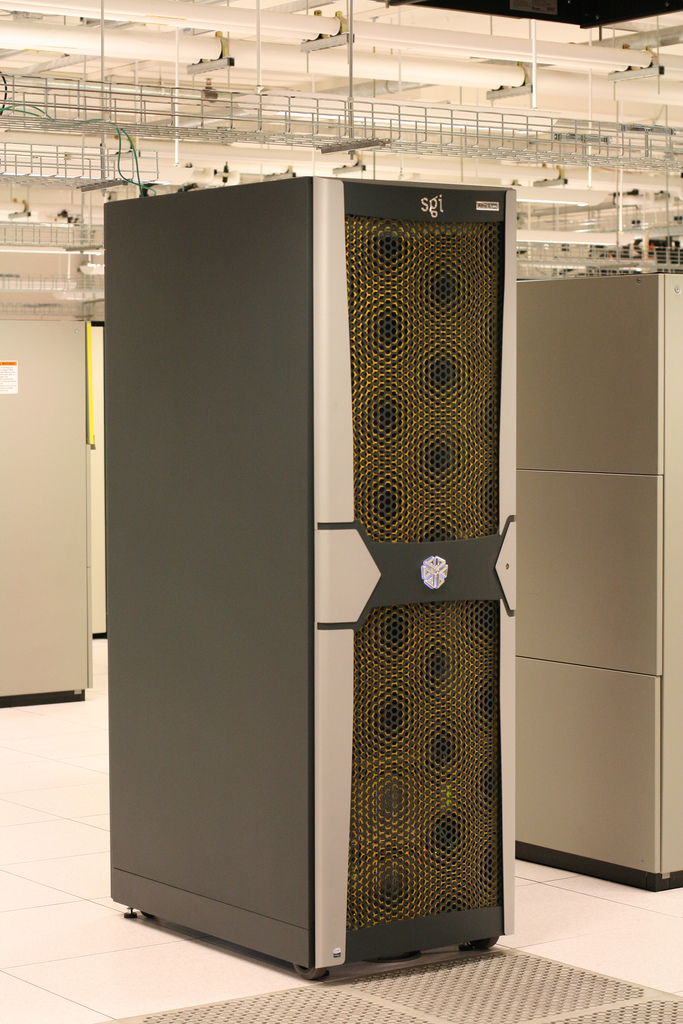
\includegraphics[height=2.7in]{tallbighouse}\end{center}
   \end{column}
   \end{columns}
  \end{frame}
%arch
  \subsection {Hardware}
  \begin{frame}{Bighouse Hardware}
   \begin{block}{Current Hardware}
   \begin{itemize}
    \item<1->Cache Coherency NonUniform Memory Access (ccNUMA)
     \note[item]<1->{Keeps cache lines in sync both good and bad\\
                     Makes for easy programming, places upper limit vs. CRAY}
    \item<2->16 CPU, 32 core Intel Itanium II's
    \item<3->Measured 5.5 Gflop/cpu running 4 way
     \note[item]<3->{HPL P=2 Q=2 N=20000, MKL no threads, MPT\\}
    \item<3->171.9 Gflop running 32 way
     \note[item]<3->{HPL P=4 Q=8 N=20000, MKL no threads, MPT\\}
    \item<4->96 GB Ram
     \note[item]<4->{2 nodes have 24GB, 6 have 8GB\\}
    \item<5->Max 41 GB/s Aggregate Memory bandwidth
    \item<6->NUMAlink4 3.2GByte/s, $~1 \mu$ Second Latency
   \end{itemize}
   \end{block}
  \end{frame}

  \section{Architecture}
  \subsection{ccNUMA}
  \begin{frame}{ccNUMA}
   \begin{center}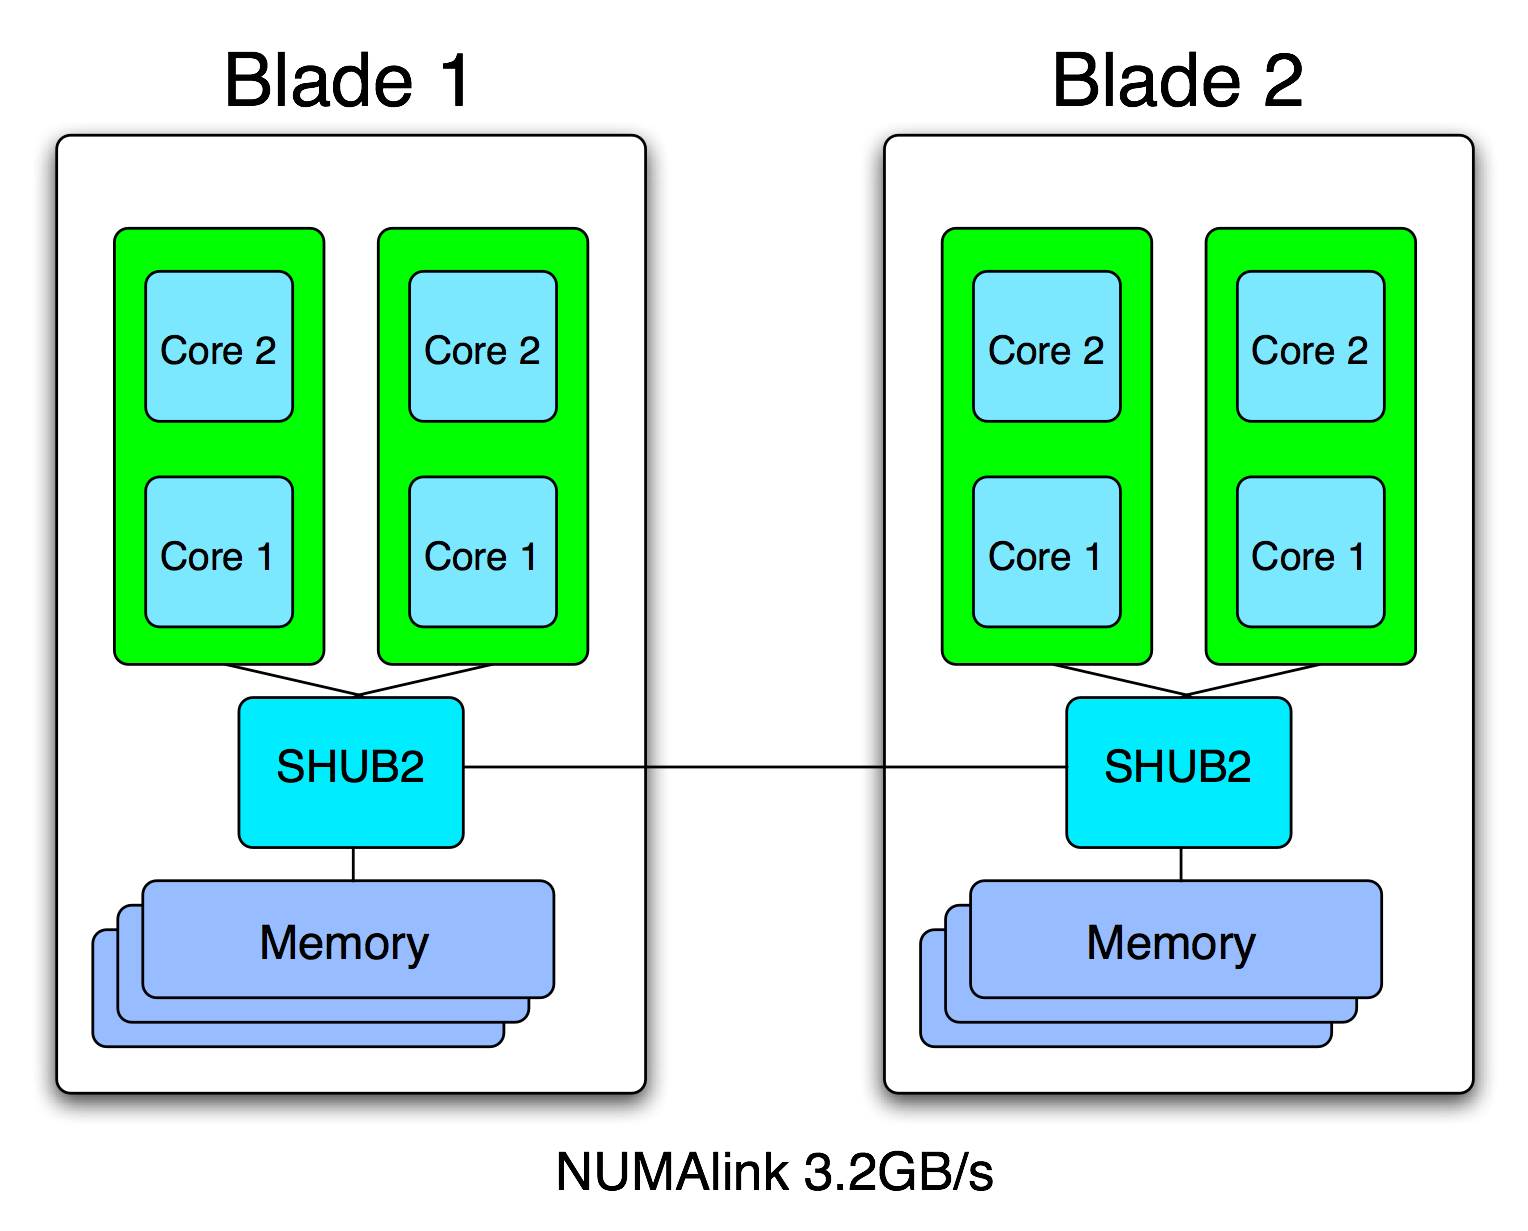
\includegraphics[height=2.5in]{numa}\end{center}
   \note[item]{Itanium II's 9000's. \\L1 16k/d 16k/i \\L2 256k/d 1024/i \\L3 4MB}
   \note[item]{SHUB2 I FORGOT IT!\\ It Sits between the cpus and memory Numa link connects to it. This is where the magic happens}
  \end{frame}
  \subsection{Altix 4700 Brick}
  \begin{frame}{Altix 4700 Brick}
   \begin{center}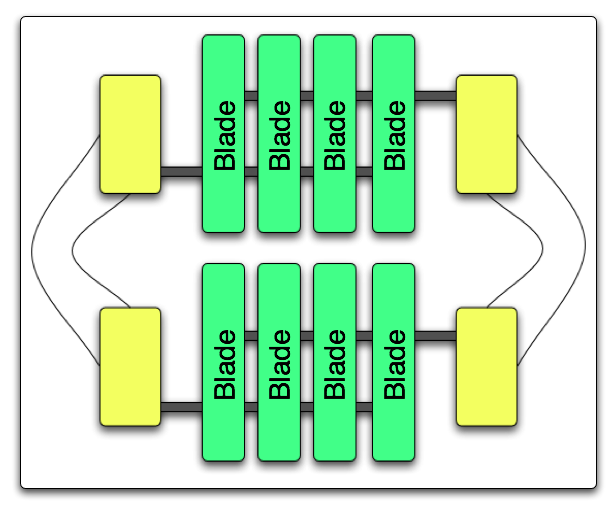
\includegraphics[height=2.5in]{bighouseBrick}\end{center}
    \note[item]{Each blade has 2 NUMAlink connections, each goes to a differnt router,  each router has a 200 nanoSec pass time.}
  \end{frame}
  \subsection{Dual Fat Tree}
  \begin{frame}{Dual Fat Tree}
   \begin{center}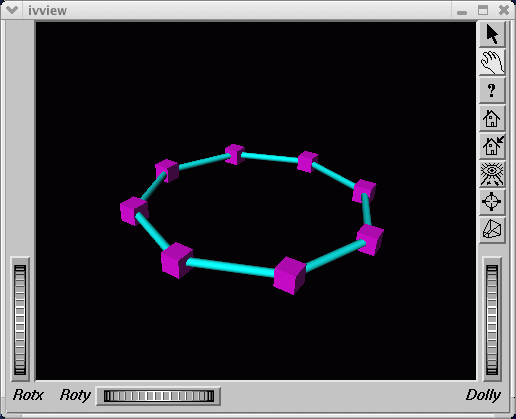
\includegraphics[height=3.0in]{ring}\end{center}
   \note[item]{This would be our layout but turns out its not\\ this would apply to the 450 if we had it.}
  \end{frame}
  \begin{frame}{Dual Fat Tree}
   \begin{center}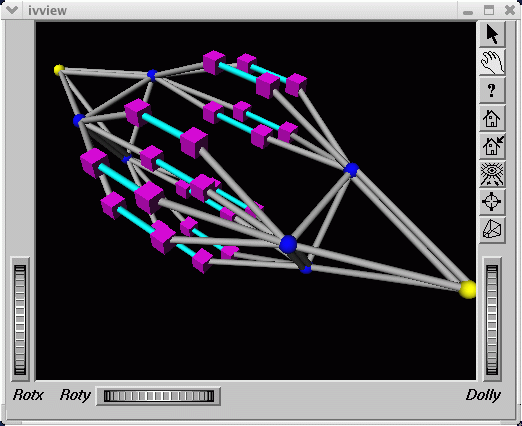
\includegraphics[height=3.0in]{16blade}\end{center}
   \note[item]{this is our layout (at 8 blades), We only have half the ring though, max number of hops will equal up to 16 blades 64 cores}
  \end{frame}
  \begin{frame}{Dual Fat Tree}
   \begin{center}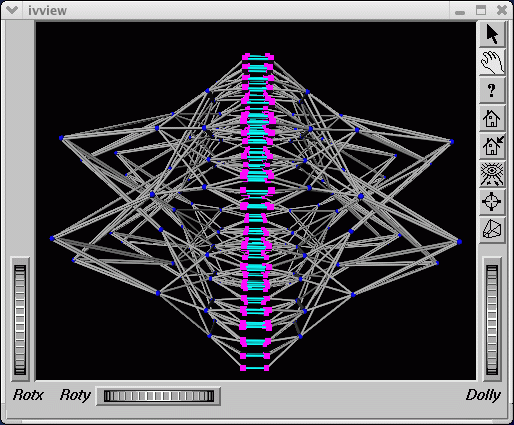
\includegraphics[height=3.0in]{256blade}\end{center}
   \note[item]{Provides 1024 cores 512 sockets\\ 
               This is the max supported config from SGI, system can add one more router out for 1024 sockets 2048 cores, MTTF is to high though}
  \end{frame}
 
\subsection{cpu sets}
\subsection{NUMA Effects}
%stream example pm graph memory use
%dlook 

\section{Software Performance}
\subsection{MPI Code}
\begin{frame}{MPT}
  \begin{block}{What is MPI?}
   \begin{itemize}
    \item <1->Message Passing Interface
    \item <2->DMP Distributed Memory Paralell
    \item <3->Hard to Program, Uses Function calls
    \item <4->Hardware is Cheap
    \item <5->Scales to 1000's of CPUS (Bluegene/L)
     \note[item]{\url{www.mpi-forum.org}}
   \end{itemize}
  \end{block}
  \begin{block}{MPT}
   \begin{itemize}
    \item <6-> MPT SGI MPI-1/2 Implementation
    \item <7-> Makes Strong Use of NUMAlink
    \item <8-> Lots of Copy on Write
     \note[item] {We have similar SM ability on nyx though OpenMPI}
   \end{itemize}
  \end{block}
\end{frame}

\begin{frame}{What is MPI?}
   \begin{center}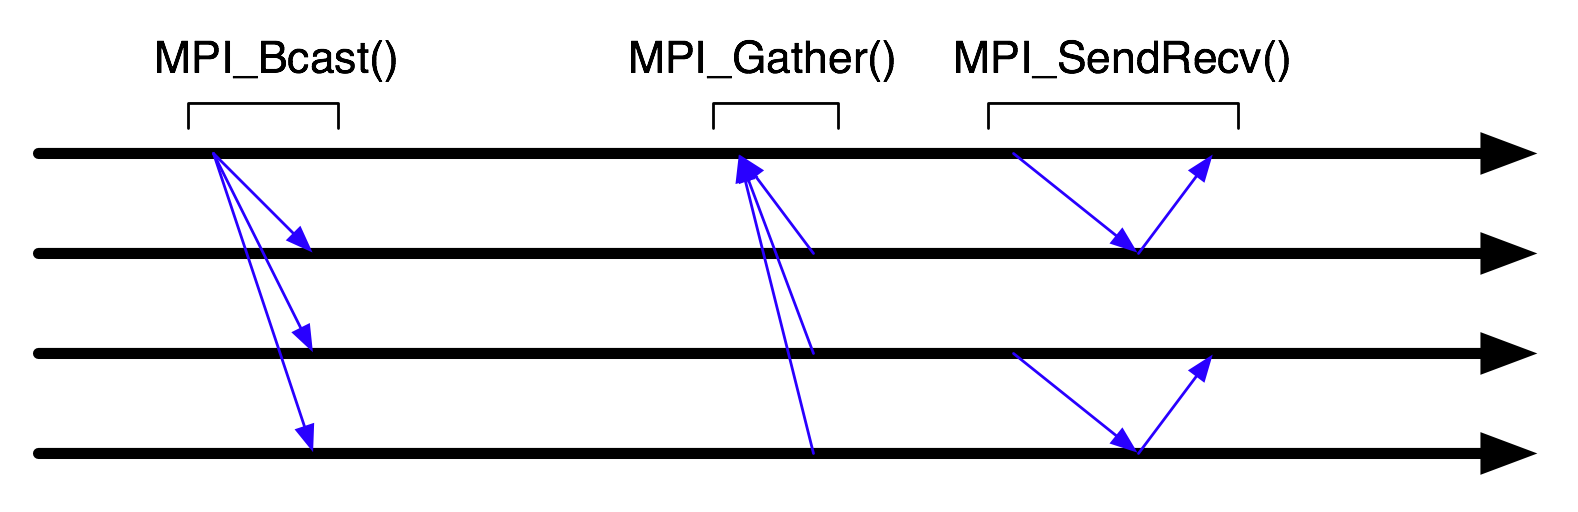
\includegraphics[height=1.5in]{mpi}\end{center}
     \note[item]{Duplicates allot of data between processes}
     \note[item]{nothing shared unless given}
\end{frame}

\begin{frame}{The Challenger}
  \begin{center}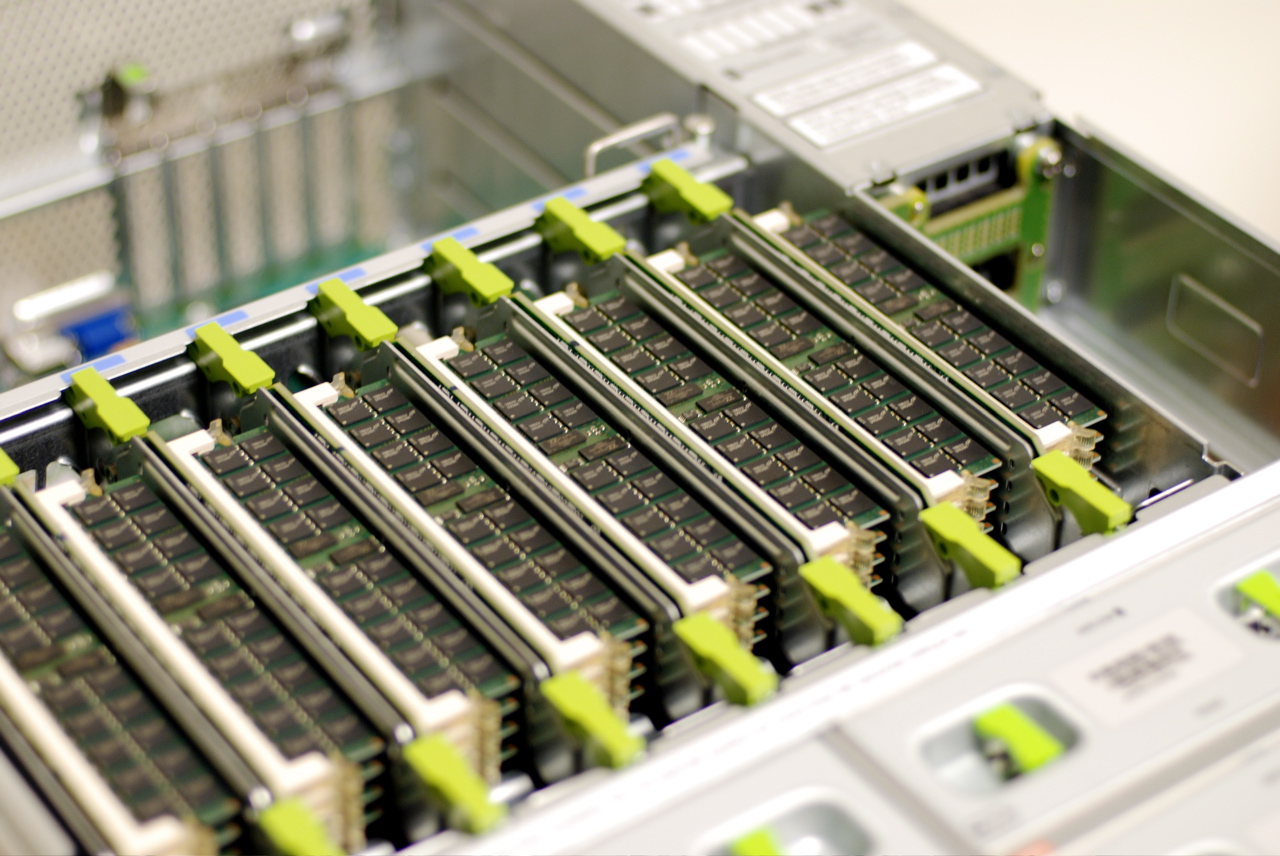
\includegraphics[height=2.5in]{jwnorman-photo01}\end{center}
   \note[item]{ \texttt{nyx801} Owned by Dr. J Norman MD, PHD. \\
                64 GB ram, on 8 sockets, dual core 8218's}
\end{frame}

\begin{frame}{MPI Perfromance/HPL}
 \begin{center}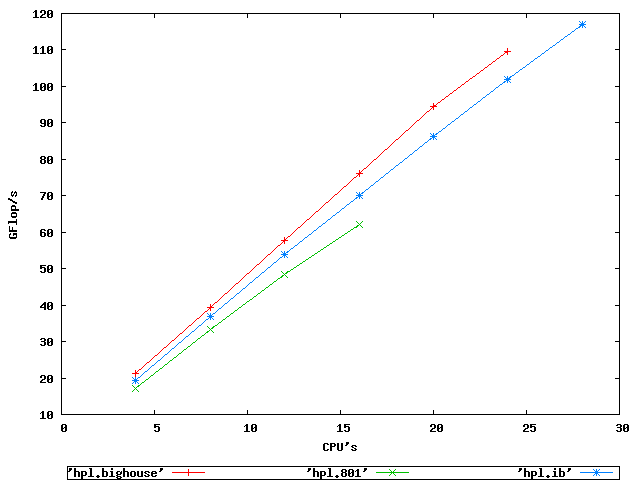
\includegraphics[height=2.5in]{hpl}\end{center}
 \note[item]{\textbf{Hardware:} \\
             'hpl.bighouse' is bighouse \\
               \begin{itemize}
		\item{mpt}
		\item{mkl no thread}
               \end{itemize}
             'hpl.801' is nyx801 \\
             'hpl.ib'  is EMike Nodes, dual core dual socket opt2220, 16 GB ram, DDR Infiniband 20Gbit/s $< 4 \mu $ Sec. Latency \\
              \begin{itemize}
 		\item{openmpi-1.2-pgi, OFED}
                \item{goto-blas}
              \end{itemize}}
 \note[item]{point out gapping as number of CPUS increase \\
             Why Bighouse is surperior, but not at this size and price}
\end{frame}

\subsection{OpenMP Code}
\begin{frame}{OpenMP}
 \begin{block}{OpenMP}
  \begin{itemize}
   \item <1->Shared Memory Parallel
   \item <2->Easy to Program, Uses Pragmas
   \item <3->Hardware is Expensive and Proprietary
   \item <4->Can Solve Any Problem (DMP or SMP)
   \item <5->Scaling Issues, Hybrid Programming
    \note[item]{Thread sync issues, implemented with libpthread normally}
   \item <6->More important with Dual/Quad/Many Core CPU's
    \note[item]{in GCC 4.1}
    \note[item]{Can FLOOD bus/interconect because of cache sync issues}
 \end{itemize}
 \end{block}
\end{frame}

\begin{frame}{OpenMP Fork and Join}
 \begin{center}
  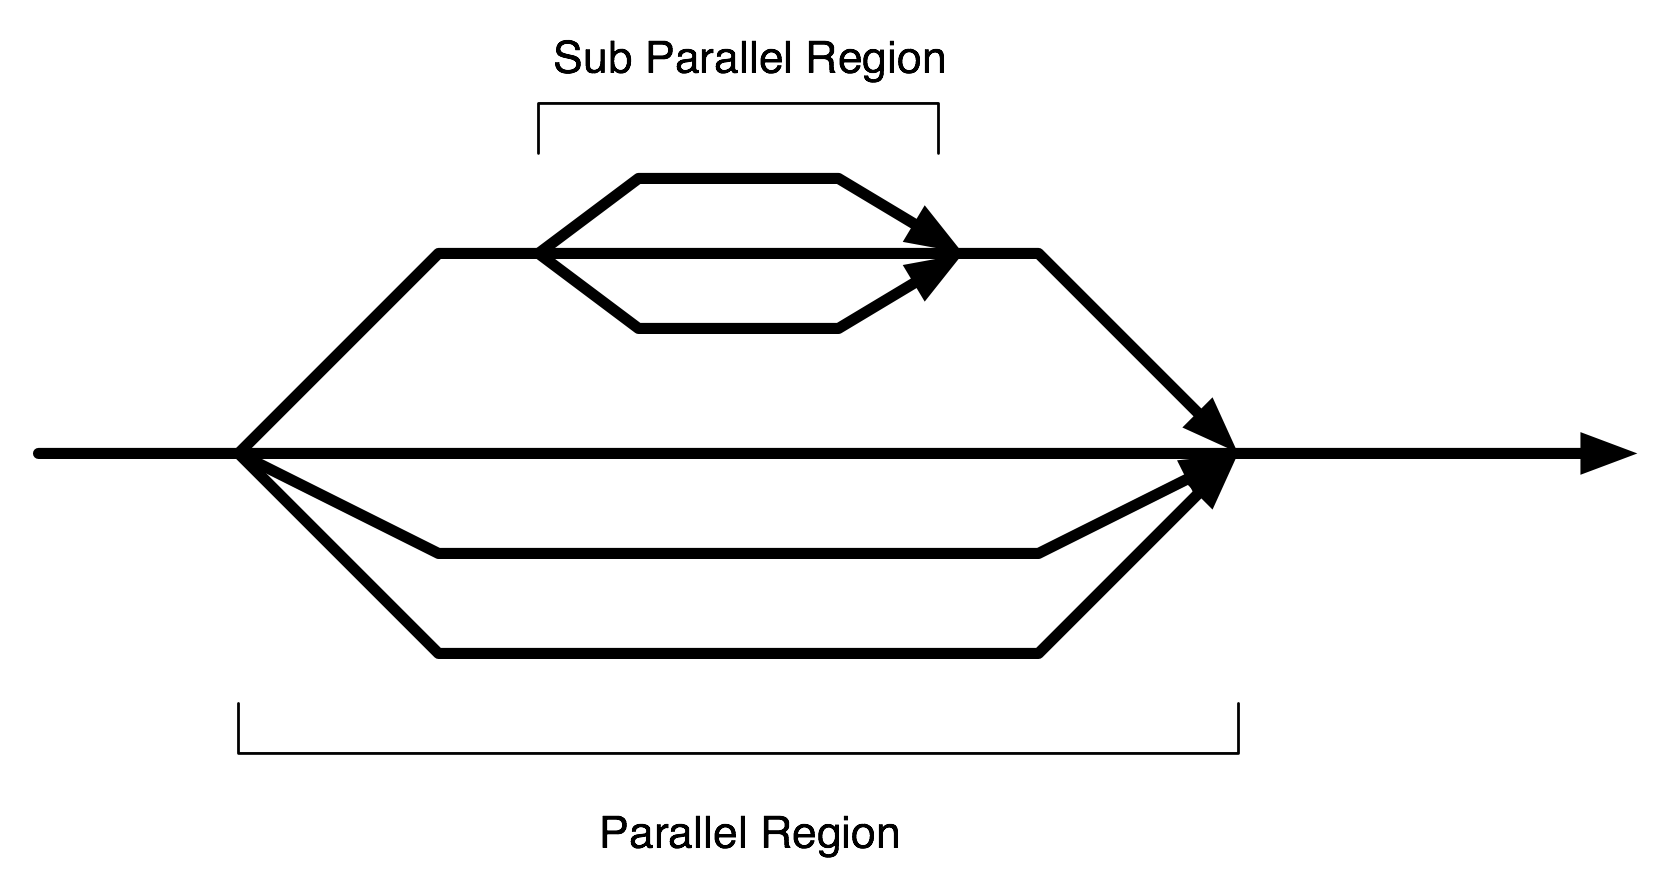
\includegraphics[height=2.5in]{openmp}
   \note[item]{This is what allot of Direct CAE apps use (Nastran Abaqus) \\
               Most interative solvers are dense matrix solvers in DMP (LS-DYNA)              }
   \note[item]{\alert{STRESS} This is bighouse's benefit, it can the ram and SMP ability to run these codes at a speed a regular cluster could never do}
 \end{center}
\end{frame}

\begin{frame}{OpenMP Performance/dgemm 36,621 MByte}
 \begin{center}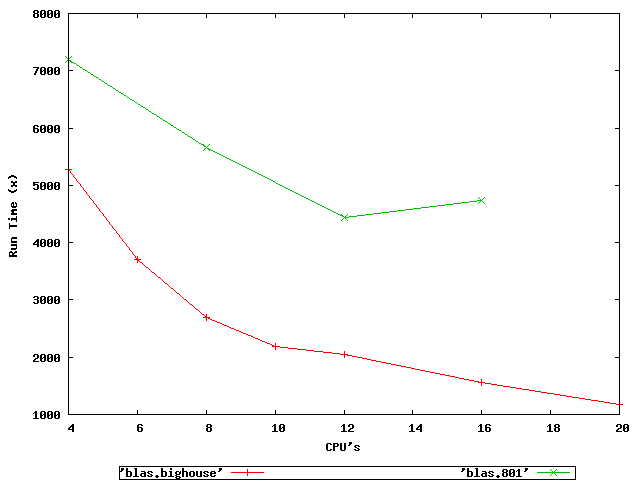
\includegraphics[height=2.5in]{blas}\end{center}
 \note[item]{\url{www.netlib.org/blas} \\
             Bighouse uses MKL \\
             nyx801 Uses ACML-pgi-mp \\
             2 equal square matrix's of random nubmers with a dim of: 40,000 Doubles. \\
             This is 3,200,000,000 (3.2 billion numbers) \\
             Same building block used in hpl
             }
\end{frame}

\begin{frame}{Example Cases}
 \begin{block}{Example Cases}
  \begin{itemize}
   \item <1-2>NUMA Memory Placement \texttt{dlook(1) dplace(1) cpuset(1)}
   \item <2>Example Cpuset OH NO SWAP
    \note{
     \begin{itemize}
     \item {\textbf{Example 1}, cpu sets}
     \item {cpuset -c brockp -f ~brockp/cpuset.conf}
     \item {echo \$\$ $>>$ /dev/cpusets/brockp/tasks}
     \end{itemize}
     }
   \item <3-4>Memory placement ccNUMA Knows where to put memory (numa\_hit numa\_miss)
   \item<4> Example \texttt{stream.c} measures memory bandwidth
    \note{
     \begin{itemize}
     \item{\textbf{Example 2}, link speeds}
     \item{\texttt{linkstat -A}}
     \item{\texttt{pmchart} numa.mem.util.used}
     \item{\texttt{pmchart} numa.link.send\_bytes}
     \item{\alert{run \texttt{stream.c}}}
    \end{itemize}
   }
  \end{itemize}
 \end{block}
\end{frame}

\begin{frame}{Questions}
 \begin{block}{Questions?}
 Questions?
 \url{http://cac.engin.umich.edu/resources/bighouse.html}
 \url{cac-support@umich.edu}
 \end{block}
\end{frame}
\end{document}
